\chapter{\label{ch3-architecture}CTA Architecture} 

\minitoc

\notes[inline,caption={}]{
	\section{Plan}
	\subsection{Topics}
	\begin{itemize}
		\item Requirements
		\item Data Levels
	\end{itemize}
	\subsection{Questions}
	\begin{itemize}
		\item ?
	\end{itemize}
}

\section{Introduction}

Due to the large scope of \gls{cta}, in both its construction and operation, a formal approach towards a system architecture was adopted \cite{Dazzi2018}. One important aspect within this architecture is the distinction between the \gls{cta} Consortium and the \gls{cta} Observatory. The \gls{cta} Consortium is a group of institutes responsible for directing the science goals of the observatory, and for developing software and hardware (including cameras), which are supplied to the observatory as in-kind contributions. The consortium consists of 200 institutes across 31 countries \cite{cta-consortium}. Conversely, the CTA Observatory pertains to the major astronomical facility that serves science data to a wide user community as an open observatory. The \gls{cta} Observatory gGmbH is the legal entity for \gls{cta} in the preparation for the implementation of the \gls{cta} Observatory, and works in close cooperation with the consortium during this process \cite{cta-observatory}.

The purpose of the \textit{\gls{cta} Architecture} is to maintain communication and understanding among all \gls{cta} contributors during the pre-construction phase in order to ensure a coherent development process and seamless integration of the developed units into a whole. During this chapter I will describe two aspects of the \textit{\gls{cta} Architecture} that are important in the context of this thesis: certain requirements that all cameras, including \gls{chec}, must meet; and the descriptions of how camera-observation data are handled in \gls{cta}, including the system flow and data level definitions.

\section{Requirements}

In order to ensure the science goals of \gls{cta} are achievable, and that the observatory remains operational for the full 30 life-time, certain standards must be upheld by all components of the observatory; this is the purpose of the \gls{cta} requirements. The requirements cover every aspect of the observatory, including: the survival of environmental conditions (\textit{B-ENV-0320 Survival humidity}), the time allowed by the analysis pipeline for processing (\textit{A-OBS-0810 Data Processing Efficiency}), the reliability of telescope components (\textit{B-TEL-0520 Structure Lifetime}), and the ability to meet the expected performance (\textit{PROG-0025 Differential Sensitivity under Low Moonlight - North}). In order for an in-kind contribution to be accepted, it must meet the requirements defined by the observatory. These requirements are therefore the standards for which we compare the performance of \gls{chec} against, and are the primary drivers in my development of the low-level calibration and analysis. However, there exists more than 60 requirements specifically tailored for the cameras. Consequently, the full review of the camera is a large undertaking that extends beyond the scope of this thesis. Instead, only the requirements that have relevance to the topic of this thesis are discussed.

It is important to note that the requirements, located on the \gls{cta} Jama website \cite{cta-jama}, are currently under-review and therefore subject to change. One such change that is under-way at the time of this writing is the redefinition from units of photoelectrons to photons. Originally, a common consolidated \gls{pmt} was envisioned to be used for all cameras in \gls{cta}, motivating for the expression of requirements to be in photoelectrons. However, due to the advances in sensor technology and the adoption of \glspl{sipmt}, this assumption has lead to problems with such a definition \cite{petophotons}. Firstly, a fixed \gls{nsb} level defined in terms of photoelectrons does not allow for trade-offs between \gls{nsb} acceptance and other performance parameters. Secondly, with an \gls{sipmt}-based camera it is possible to obtain a better Cherenkov intensity resolution and a lower energy threshold, but still fail the current requirements, whilst a camera design with inferior performance may pass. The current requirements could be met by a camera with subpar \glspl{sipmt} by reducing its bias voltage, which in turn reduces the optical cross-talk and photon detection efficiency, hence bringing the excess noise factor and threshold in photoelectron units down\change{talk with Tom about this, and how trigger efficiency was affected by being defined in p.e.}. While such a camera meets the current requirements, it is at the cost of performance in terms of photon intensity (and therefore Cherenkov-shower energy threshold). 

A copy of each requirement at the time of this writing is included alongside the discussion in this section to ensure clarity about which version of the requirement definition is being referred to. Future investigations should check the latest requirement definition. \vfill

\begin{requirement}{\subsection{B-TEL-1010 Charge Resolution}}
	The required fractional Charge Resolution for Cherenkov signals in each Camera pixel for a specified background level of 0.125 photoelectrons/ns is given in the Figure below and Table attached. Charge measurements must be possible for 0-1000 photoelectron signals. The average charge resolution should be calculated for the reference Gamma-Ray Spectrum.
    
	\centering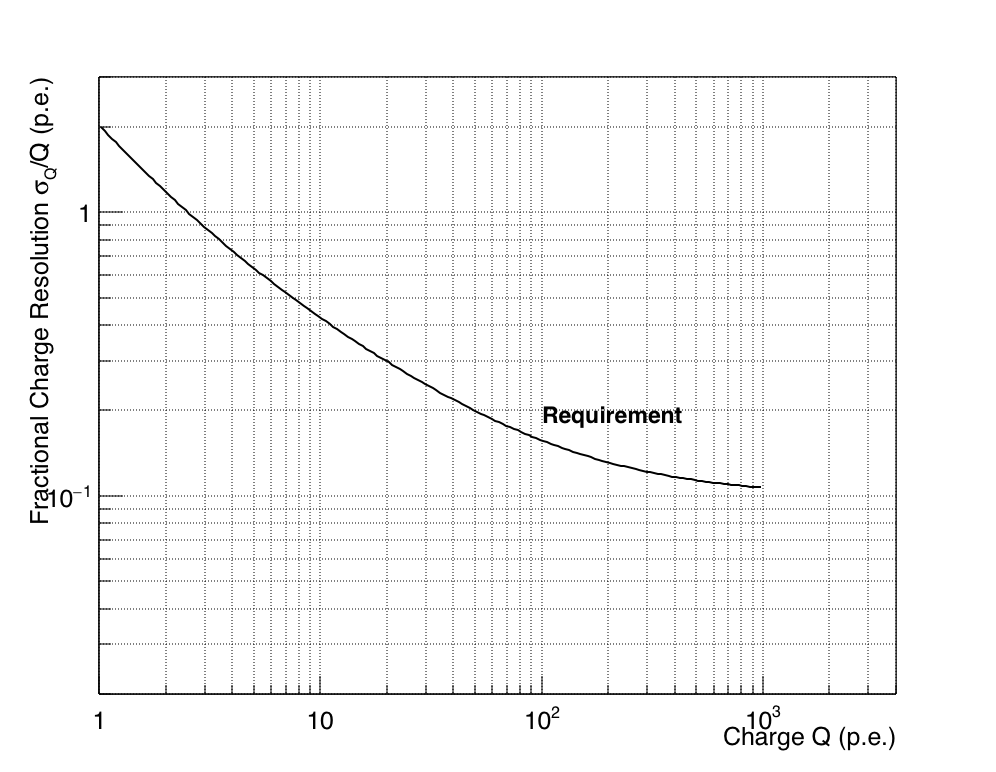
\includegraphics[width=0.8\linewidth]{charge_res_req}
	\captionof{figure}{Fractional rms charge resolution $\sigma_Q/Q$ per pixel for different Cherenkov light signal amplitudes, expressed in units of photoelectrons (p.e.). All sources of fluctuations, including Poisson fluctuations in photoelectron number, must be included, The true pixel charge $Q$ is that measured in an ideal detector with the same photon-detection efficiency. }\label{fig:charge_res_req}
    
\begin{itemize}
\item [Notes:] It is expected that this requirement is verified with reference to:

- Monte Carlo simulation of Cherenkov light from gamma-ray initiated showers (using a verified telescope model),

- Level-C Specification on Laboratory Measured Charge Resolution,

- Monte Carlo simulation of the laboratory test set-up (as a means of telescope model verification).

Note that between 1000~p.e. and 2000~p.e., some sensitivity to increasing input signal must exist. \newline
This requirement applies to post-calibration (DL1) data. \newline
Note that this requirement will likely need to be expanded to cover performance at higher NSB levels.
\end{itemize}
\end{requirement}

\subsubsection{Definition}
The standard criterion for low-level performance used in \gls{cta} is the \textit{Charge Resolution}. It encompasses both the bias and the standard deviation of the extracted charge versus the expected charge to provide a measure of the waveform, calibration, and charge reconstruction quality. Analogous to the Root-Mean-Square Error, the fractional \textit{Charge Resolution} $\dfrac{\sigma_Q}{Q_T}$ for a particular ``true charge'' $Q_T$ (the charge that would be measured directly after the photocathode of the sensor) is defined as
\begin{equation} \label{eq:charge_res}
\dfrac{\sigma_Q}{Q_T} = \dfrac{1}{Q_T} \sqrt{\dfrac{\sum_{i=0}^N (Q_{M_i} - Q_T)^2}{N}},
\end{equation}
where $N$ is the total number of measured charges, $Q_{M_i}$, with that value of $Q_T$. The associated \gls{cta} requirement defines the maximum allowed values of $\dfrac{\sigma_Q}{Q_T}$ for values of $Q_T$ between 1-1000~p.e., which must be adhered to when resolving the signal for any camera in \gls{cta}.

\subsubsection{Requirement Derivation}
The uncertainty in charge reconstruction can be expressed in the form
\begin{equation} \label{eq:charge_res_req}
\dfrac{\sigma_Q}{Q} = \dfrac{1}{Q} \sqrt{\sigma_0^2 + \sigma_{ENF}^2 Q + \sigma_g^2 Q^2},
\end{equation}
where $\sigma_0$ encapsulates noise contributions (electronic and \gls{nsb}), $\sigma_{ENF} = 1 + \mathit{ENF}$ is determined from the \textit{Excess Noise Factor} (a measure of the avalanche gain fluctuations), and $\sigma_g$ is the multiplicative errors of the gain \cite{petophotons}\cite{Ohm2012}. $\sigma_0$ can be further expanded in terms of the two primary noise contributions:
\begin{equation} \label{eq:charge_res_nsb}
\sigma_0 = \sqrt{\mathit{NSB} \times t_w + n_e^2},
\end{equation}
i.e. the $\mathit{NSB}$ rate (which includes the \gls{dcr} for the purpose of this discussion) is coupled with the effective signal readout window size, $t_w = 15$ ns, and summed with the electronic noise, $n_e$. A contribution from electronic noise of $n_e = 0.87$ photoelectrons is assumed, combined with a value of $\mathit{NSB} = 0.125$ p.e./ns as defined in the requirement. A value of $\sigma_g = 0.1$ and $\mathit{ENF} = 0.2$ is also assumed \cite{petophotons}. The resulting combination of miscalibration and noise factors in Equation~\ref{eq:charge_res_req} gives the \textit{Charge Resolution} requirement illustrated in Figure~\ref{fig:charge_res_req}.

\subsubsection{Approach}
As it is impossible to know the ``true charge'' generated by a Cherenkov signal in the field, Monte Carlo simulations must be relied upon in order to prove a camera meets this requirement. The process for achieving this is outlined in the notes to the requirement. It is expected that this requirement is validated in three ways:
\begin{enumerate}
\item With lab measurements where the camera in uniformly illuminated with a calibrated light-source.
\item With simulations of the previous approach, in order to verify the simulation model of the camera.
\item With Monte Carlo simulations of Cherenkov signal incident on the full telescope model.
\end{enumerate}
The final item is the most important in confirming the requirements are met, as temporally-uniform illuminations do not sufficiently test the ability to find the signal pulse in the waveforms for the case of a Cherenkov-shower illumination. 

The software package \textit{sim\_telarray} (Chapter~\ref{ch4-software}) stores the ``true charge'' generated after the photocathode for each shower event into the output file. Therefore, with an accurately simulation model of the camera, it is an appropriate package for investigating a camera's performance against this requirement. However, in order to ensure Poisson fluctuations in photoelectron number are included, as per the requirement, when using the ``true charge'' stored in the simulation file, the corrected form of Equation~\ref{eq:charge_res} is
\begin{equation} \label{eq:charge_res2}
\dfrac{\sigma_Q}{Q_T} = \dfrac{1}{Q_T} \sqrt{\dfrac{\sum_{i=0}^N (Q_{M_i} - Q_T)^2}{N} + Q_T}.
\end{equation}
With the form in Equation~\ref{eq:charge_res2}, a perfect detector that consistently reads-out a ``measured charge'' with equal value to the ``true charge'' would hit the Poisson limit, as it is not physically possible to know the the ``true charge'' generated by the photocathode without fluctuations. The Poisson limit is shown alongside the \textit{Charge Resolution} requirement in Figure~\change{figure showing the two limit lines}.
\newline
\begin{requirement}{\subsection{B-TEL-1295 Pixel Availability}}
During observations, at least 95\% of all camera pixels must be available and usable for data analysis. In addition, continuous regions of non-functioning pixels must not exceed 2\% of all camera pixels. Pixels excluded due to NSB levels beyond those required are not included in this budget.
\end{requirement}

This requirement sets a limit on the amount of ``dead'' pixels that can be allowed on a camera before the entire camera is considered to be unavailable. For \gls{chec}, which contains 2048 pixels, this imposes the following possible limitations:
\begin{itemize}
\item The camera may only have a maximum of 102 dead pixels. This allows 3 dead pixels per module.
\item The amount of continuous pixels that are allowed to be dead is 41, therefore if a module dies, the camera's capabilities become insufficient for the \gls{cta} requirements. However, a maximum of two \glspl{asic} are allowed to die.
\end{itemize}

\section{Data Level and Flow Model}

\begin{figure}
  \centering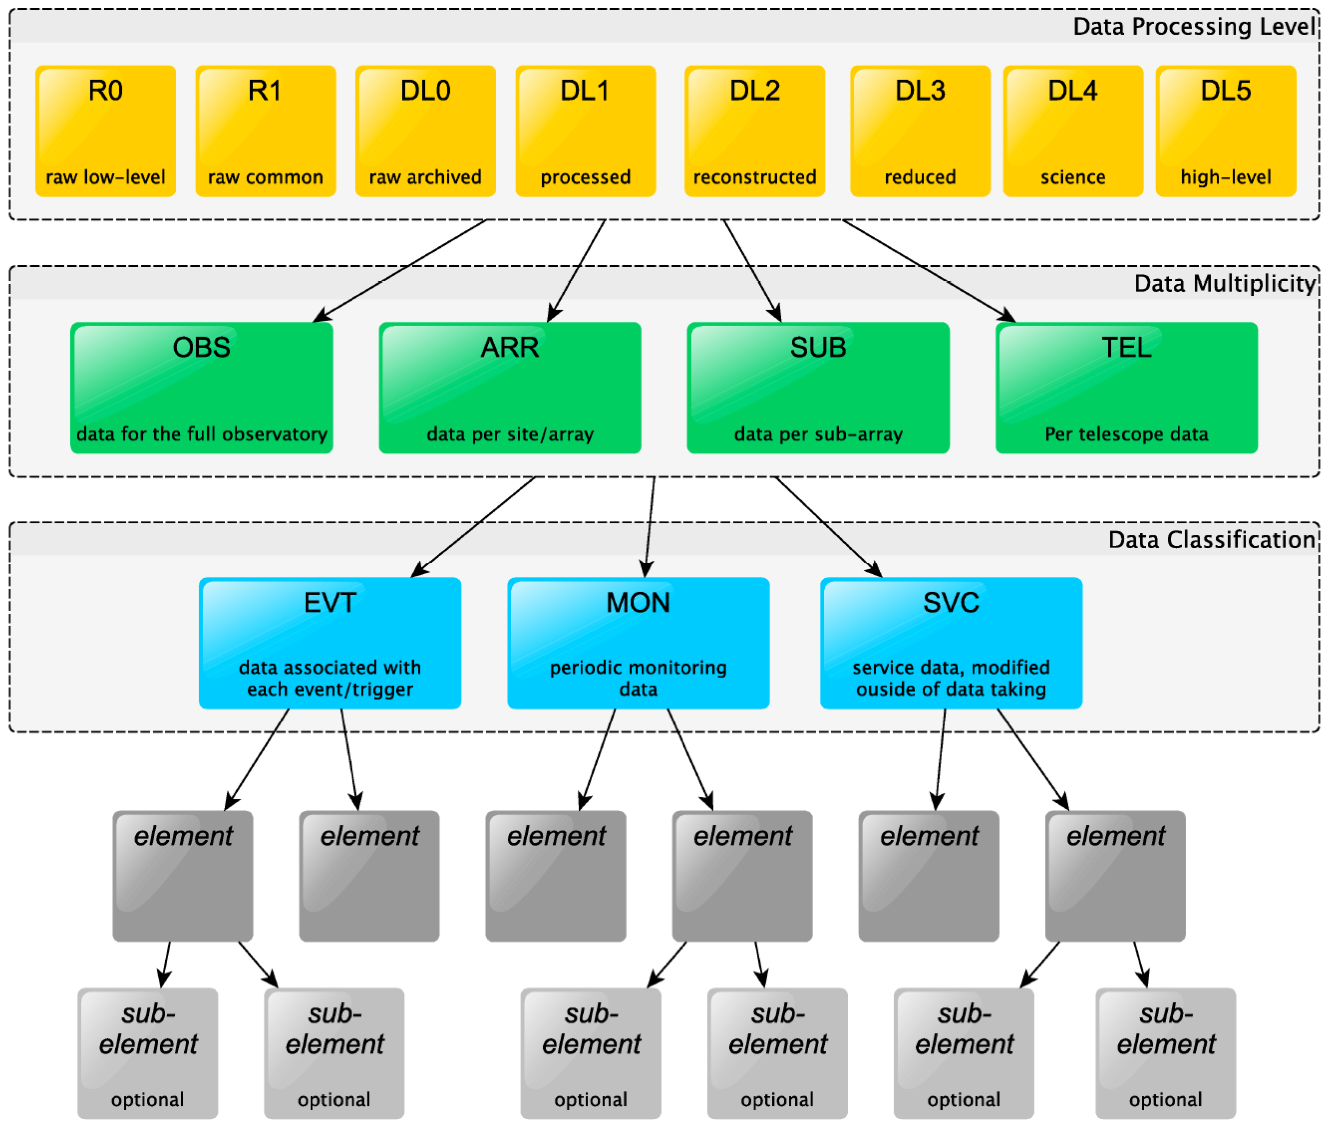
\includegraphics[width=\textwidth]{high_level_data_model} 
	\caption[High-level Data Model Hierarchy]{Hierarchy of data element names including the data level, the classifications of data (based on their rate), and data elements/groups and sub-elements/groups \cite{Kosack2017}.}
	\label{fig:high_level_data_model}
\end{figure}

Another aspect of the \textit{\gls{cta} Architecture} that is relevant to this work are the \textit{Data Processing Level} definitions, and the flow between them. These definitions dictate how the data obtained from the telescopes are handled within the observatory, and are important in ensuring each telescope adopts a similar processing chain to guarantee compatibility between themselves and the pipeline framework software.

Figure~\ref{fig:high_level_data_model} shows the full hierarchy for data specification in the observatory. The \textit{Data Processing Level} indicates the progression of the data along the processing chain, the \textit{multiplicity} indicates the scope of the data, and the \textit{classification} designates the type of the data \cite{Kosack2017}. As the primary focus of this thesis is on the individual telescopes waveform data, the rest of this section will be focussed on describing the data levels relevant to the \textit{EVT}- classification, and the processes used to transition between them. This subject is still undergoing development within \gls{cta}, but the foundations are generally accepted. A simple overview of this topic is shown in Figure~\ref{dataflow}.

\begin{wrapfigure}[36]{r}{0.32\textwidth}
  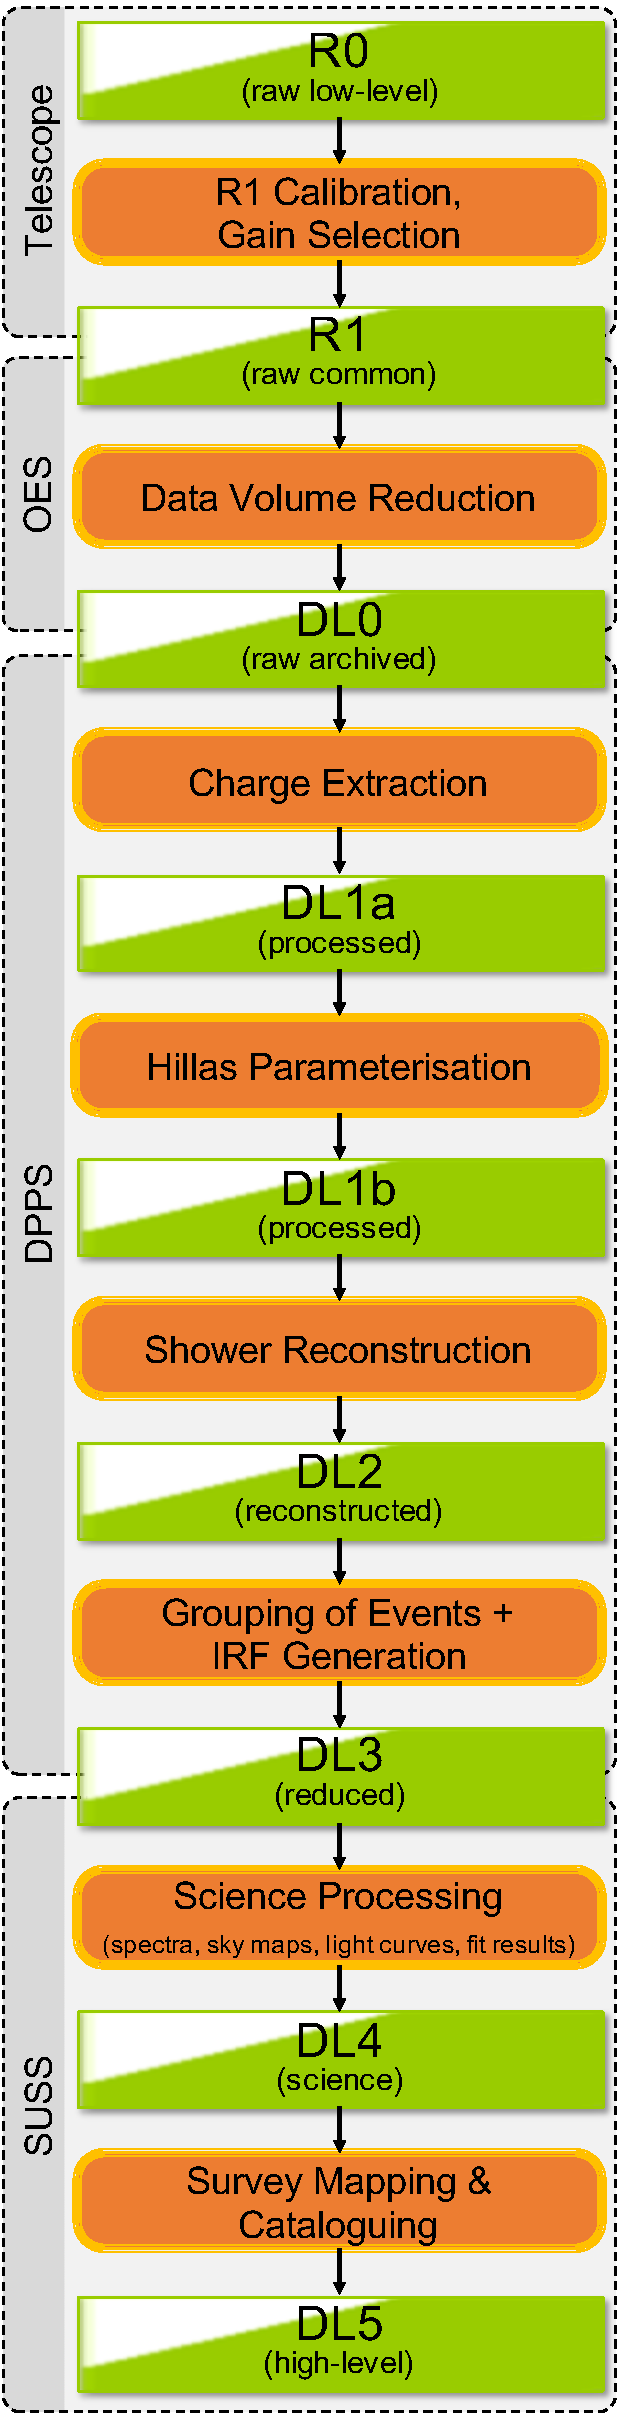
\includegraphics[width=0.32\textwidth]{dataflow}
  \caption{Simplified camera data flow, showing the \textit{EVT}-classified data streams (in green) and
the processing steps between them (orange). The levels are grouped by the systems responsible for them.}\label{fig:dataflow}
\end{wrapfigure}

\textbf{R0} \textit{(raw low-level)}:
Raw waveform data, internal to the Camera Functional Unit.

\textbf{R1} \textit{(raw common)}:
Waveform data with \textit{R1 Calibration} applied. This low-level calibration is unique to the camera, to remove the dependence on the behaviour of its specific electronics. The \gls{chec} \textit{R1 Calibration} is described in Chapter~\ref{ch5-calibration}. A selection of gain-channel is also performed for cameras with 2 channels. This level contains data which are serialised to a wire format, i.e. a block of data sent over a network in a common way between the telescopes. This data level is processed by the \textit{Online Analysis} pipeline in order to produce immediate science alerts. The \textit{R1} level therefore has its own \textit{\gls{cta} Requirements} to adhere to (including its own \textit{Charge Resolution} requirement), ensuring that the minimum standard required for the \textit{Online Analysis} and \textit{Data Volume Reduction} is met. Further (potentially slower) calibration may be applied at a later stage (\textit{DL0} to \textit{DL1a}) such that the results of the offline pipeline are of optimum quality.

\textbf{DL0} \textit{(raw archived)}: Similar data to the \textit{R1} level, except serialised into files and are intended to be archived for the long-term. In order to achieve this with the excessively large data volume produced by \gls{cta}, \textit{Data Volume Reduction} must be performed to achieve 2 orders of magnitude reduction. The simplest form of reduction is known as zero-suppression, where only waveforms of pixels deemed to have signal are kept, but more advanced forms of reduction are under investigation\change{find reference}. This is one of the responsibilities of the Observation Execution System (OES).

\textbf{DL1} \textit{(processed)}: The signal charge is extracted from the \textit{DL0} waveform data, and characterised in terms of its \textit{Hillas Parameters}. This process is handled by the Data Processing and Preservation System (DPPS) offline data processing pipeline, of which \pkg{ctapipe} is a prototype of. Further information about \pkg{ctapipe} can be found in Chapter~\ref{ch4-software}, and details about the processes in this stage are described in Chapter~\ref{ch6-reduction}.

\textbf{DL2} \textit{(reconstructed)}: The \textit{DL1} products (pixel charges and \textit{Hillas Parameters}) are used to reconstruct shower parameters including energy, direction, and source particle. At this point, the \textit{TEL multiplicity} is dropped, as the information from each telescope has been combined to perform the reconstruction, and the individual telescopes are no longer relevant. The operations involved in this stage are also performed by the DPPS offline pipeline, and are described in Chapter~\ref{ch6-reduction}.

\textbf{DL3} \textit{(reduced)}:
Events are sorted into sets according to their type (e.g. gamma-ray candidates, electron candidates, selected hadron
candidates, etc.) alongside their reconstruction parameters. Associated instrumental response characterizations and any technical data needed for
science analysis are also included in this level.

\textbf{DL4} \textit{(science)}:
The \textit{DL3} data are read into the one of  the CTA tools within the Science User Support System (SUSS) designed to support science data analysis. Two prototype tools developed within this system are \textit{gammapy} and \textit{ctools} (Chapter~\ref{ch4-software}). These tools provide enable the construction of binned data products like spectra, sky maps, or light curves. These can be fit against models to make conclusions about the astronomical source.

\textbf{DL5} \textit{(high-level)}:
Accumulations of \textit{DL4} data to generate \gls{cta} survey sky maps or the \gls{cta}
source catalogue.